\documentclass[10pt,twoside,a4paper]{article}

% Configure these parameters.
% Name and email
\newcommand{\studentname}{Joe Yan}
\newcommand{\studentemail}{zy275@cam.ac.uk}

% Date work done
\newcommand{\svworkdate}{2016-10-17}

% Details of supervision
\newcommand{\svcourse}{CST Part IA: Digital Design}
\newcommand{\svnumber}{2}
\newcommand{\svdate}{2016-10-22}
\newcommand{\svtime}{15:30}
\newcommand{\svvenue}{Churchill Seminar Room 1}
\newcommand{\svrname}{Mr Matthew Ireland}
\newcommand{\svrinit}{JKF}
% End configuration

\usepackage{a4}             % Adjust margins for A4 media
\usepackage{fancyhdr}
\renewcommand{\headrulewidth}{0.4pt}
\renewcommand{\footrulewidth}{0.4pt}
\fancyheadoffset[LO,LE,RO,RE]{0pt}
\fancyfootoffset[LO,LE,RO,RE]{0pt}
\pagestyle{fancy}
\fancyhead{}
\fancyhead[LO,RE]{{\bfseries \studentname}\\\studentemail}
\fancyhead[RO,LE]{{\bfseries \svcourse, SV~\svnumber}\\\svdate\ \svtime, \svvenue}
\fancyfoot{}
\fancyfoot[LO,RE]{For: \svrname}
\fancyfoot[RO,LE]{\thepage\ / \pageref{LastPage}}
\fancyfoot[C]{\today}

\usepackage{lastpage}       % "n of m" page numbering
\usepackage{lscape}         % Makes landscape easier
%\usepackage{portland}      % Switch between portrait and landscape
\usepackage{graphics}       % Graphics commands
\usepackage{wrapfig}        % Wrapping text around figures
\usepackage{epsfig}         % Embed encapsulated postscript
\usepackage{rotating}       % Extra graphics rotation
%\usepackage{tables}        % Tabular environments
\usepackage{longtable}      % Page breaks within tables
\usepackage{supertabular}   % Page breaks within tables
\usepackage{multicol}       % Allows table cells to span cols
\usepackage{multirow}       % Allows table cells to span rows
\usepackage{texnames}       % Macros for common tex names
%\usepackage{trees}         % Tree-like layout
\usepackage{hhline}         % Horizontal lines in tables
\usepackage{siunitx}        % Correct spacing of units

\usepackage{listings}       % Source code listings
\usepackage{array}          % Array environment
\usepackage{hyperref}       % URL formatting
\usepackage{amsmath}        % American Mathematical Society
\usepackage{amssymb}        % Maths symbols
\usepackage{amsthm}         % Theorems
%\usepackage{mathpartir}    % Proofs and inference rules
\usepackage{verbatim}       % Verbatim blocks
\usepackage{ifthen}         % Conditional processing in tex
\usepackage{xcolor}         % X11 colour names

% control width and vertically align text in table cells
\newcolumntype{L}[1]{>{\raggedright\let\newline\\\arraybackslash\hspace{0pt}}m{#1}}
\newcolumntype{C}[1]{>{\centering\let\newline\\\arraybackslash\hspace{0pt}}m{#1}}
\newcolumntype{R}[1]{>{\raggedleft\let\newline\\\arraybackslash\hspace{0pt}}m{#1}}

% make hyperref links not-ugly
\hypersetup{
    colorlinks=false,
    pdfborder={0 0 0},
}

\renewcommand{\oddsidemargin}{-20pt}
\renewcommand{\evensidemargin}{-20pt}
\renewcommand{\topmargin}{-30pt}
\renewcommand{\textwidth}{410pt}
\renewcommand{\marginparwidth}{100pt}

\setlength{\parindent}{0em}
\addtolength{\parskip}{1ex}

\usepackage[draft]{changes}
\setauthormarkup[left]{\textbf{[#1]}~}
\definechangesauthor[\svrname]{\svrinit}{orange}
\newcommand{\jkfadd}[1]{\added[\svrinit]{#1}}
\newcommand{\jkfdel}[1]{\deleted[\svrinit]{#1}}
\newcommand{\jkfrep}[2]{\replaced[\svrinit]{#1}{#2}}
\newcommand{\jkfmar}[1]{\marginpar{\jkfadd{#1}}}

\begin{document}

\author{\studentname}
\title{\svcourse, SV~\svnumber}
\date{\svworkdate}

\textbf{\svcourse, SV~\svnumber}\\
\textbf{\studentname}\\
\textbf{\svworkdate}\\

\section*{Exercise 1}

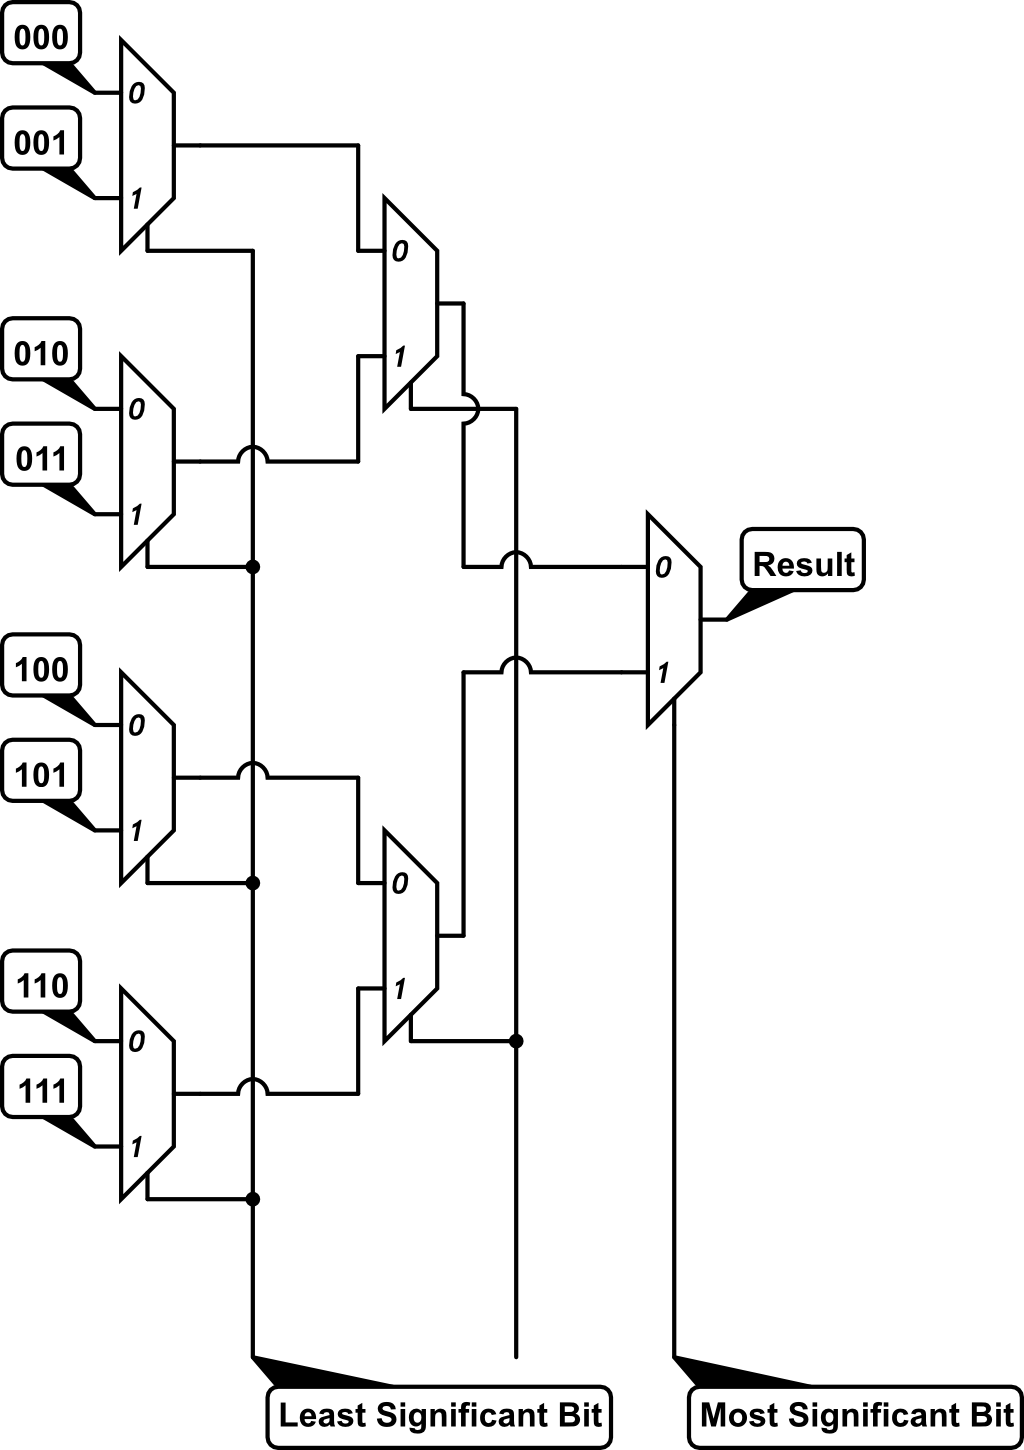
\includegraphics[scale=0.9]{sv2-1.png} 

The idea is once a control input of a "higher level" multiplexor is chosen either 0 or 1 then it is actually looking up the corresponding input from a "lower level" multiplexor output. And this idea goes through the whole circuit until get the lowest level multiplexor and take the 1 or 0 from the input. In this way,the control input of the highest level multiplexor is controlling the most significant bit of the truth table and the lowest one is controlling the least significant bit. \\
And the picture shows how it is built.

\section*{Exercise 2}
\begin{enumerate}
\item[(a)]
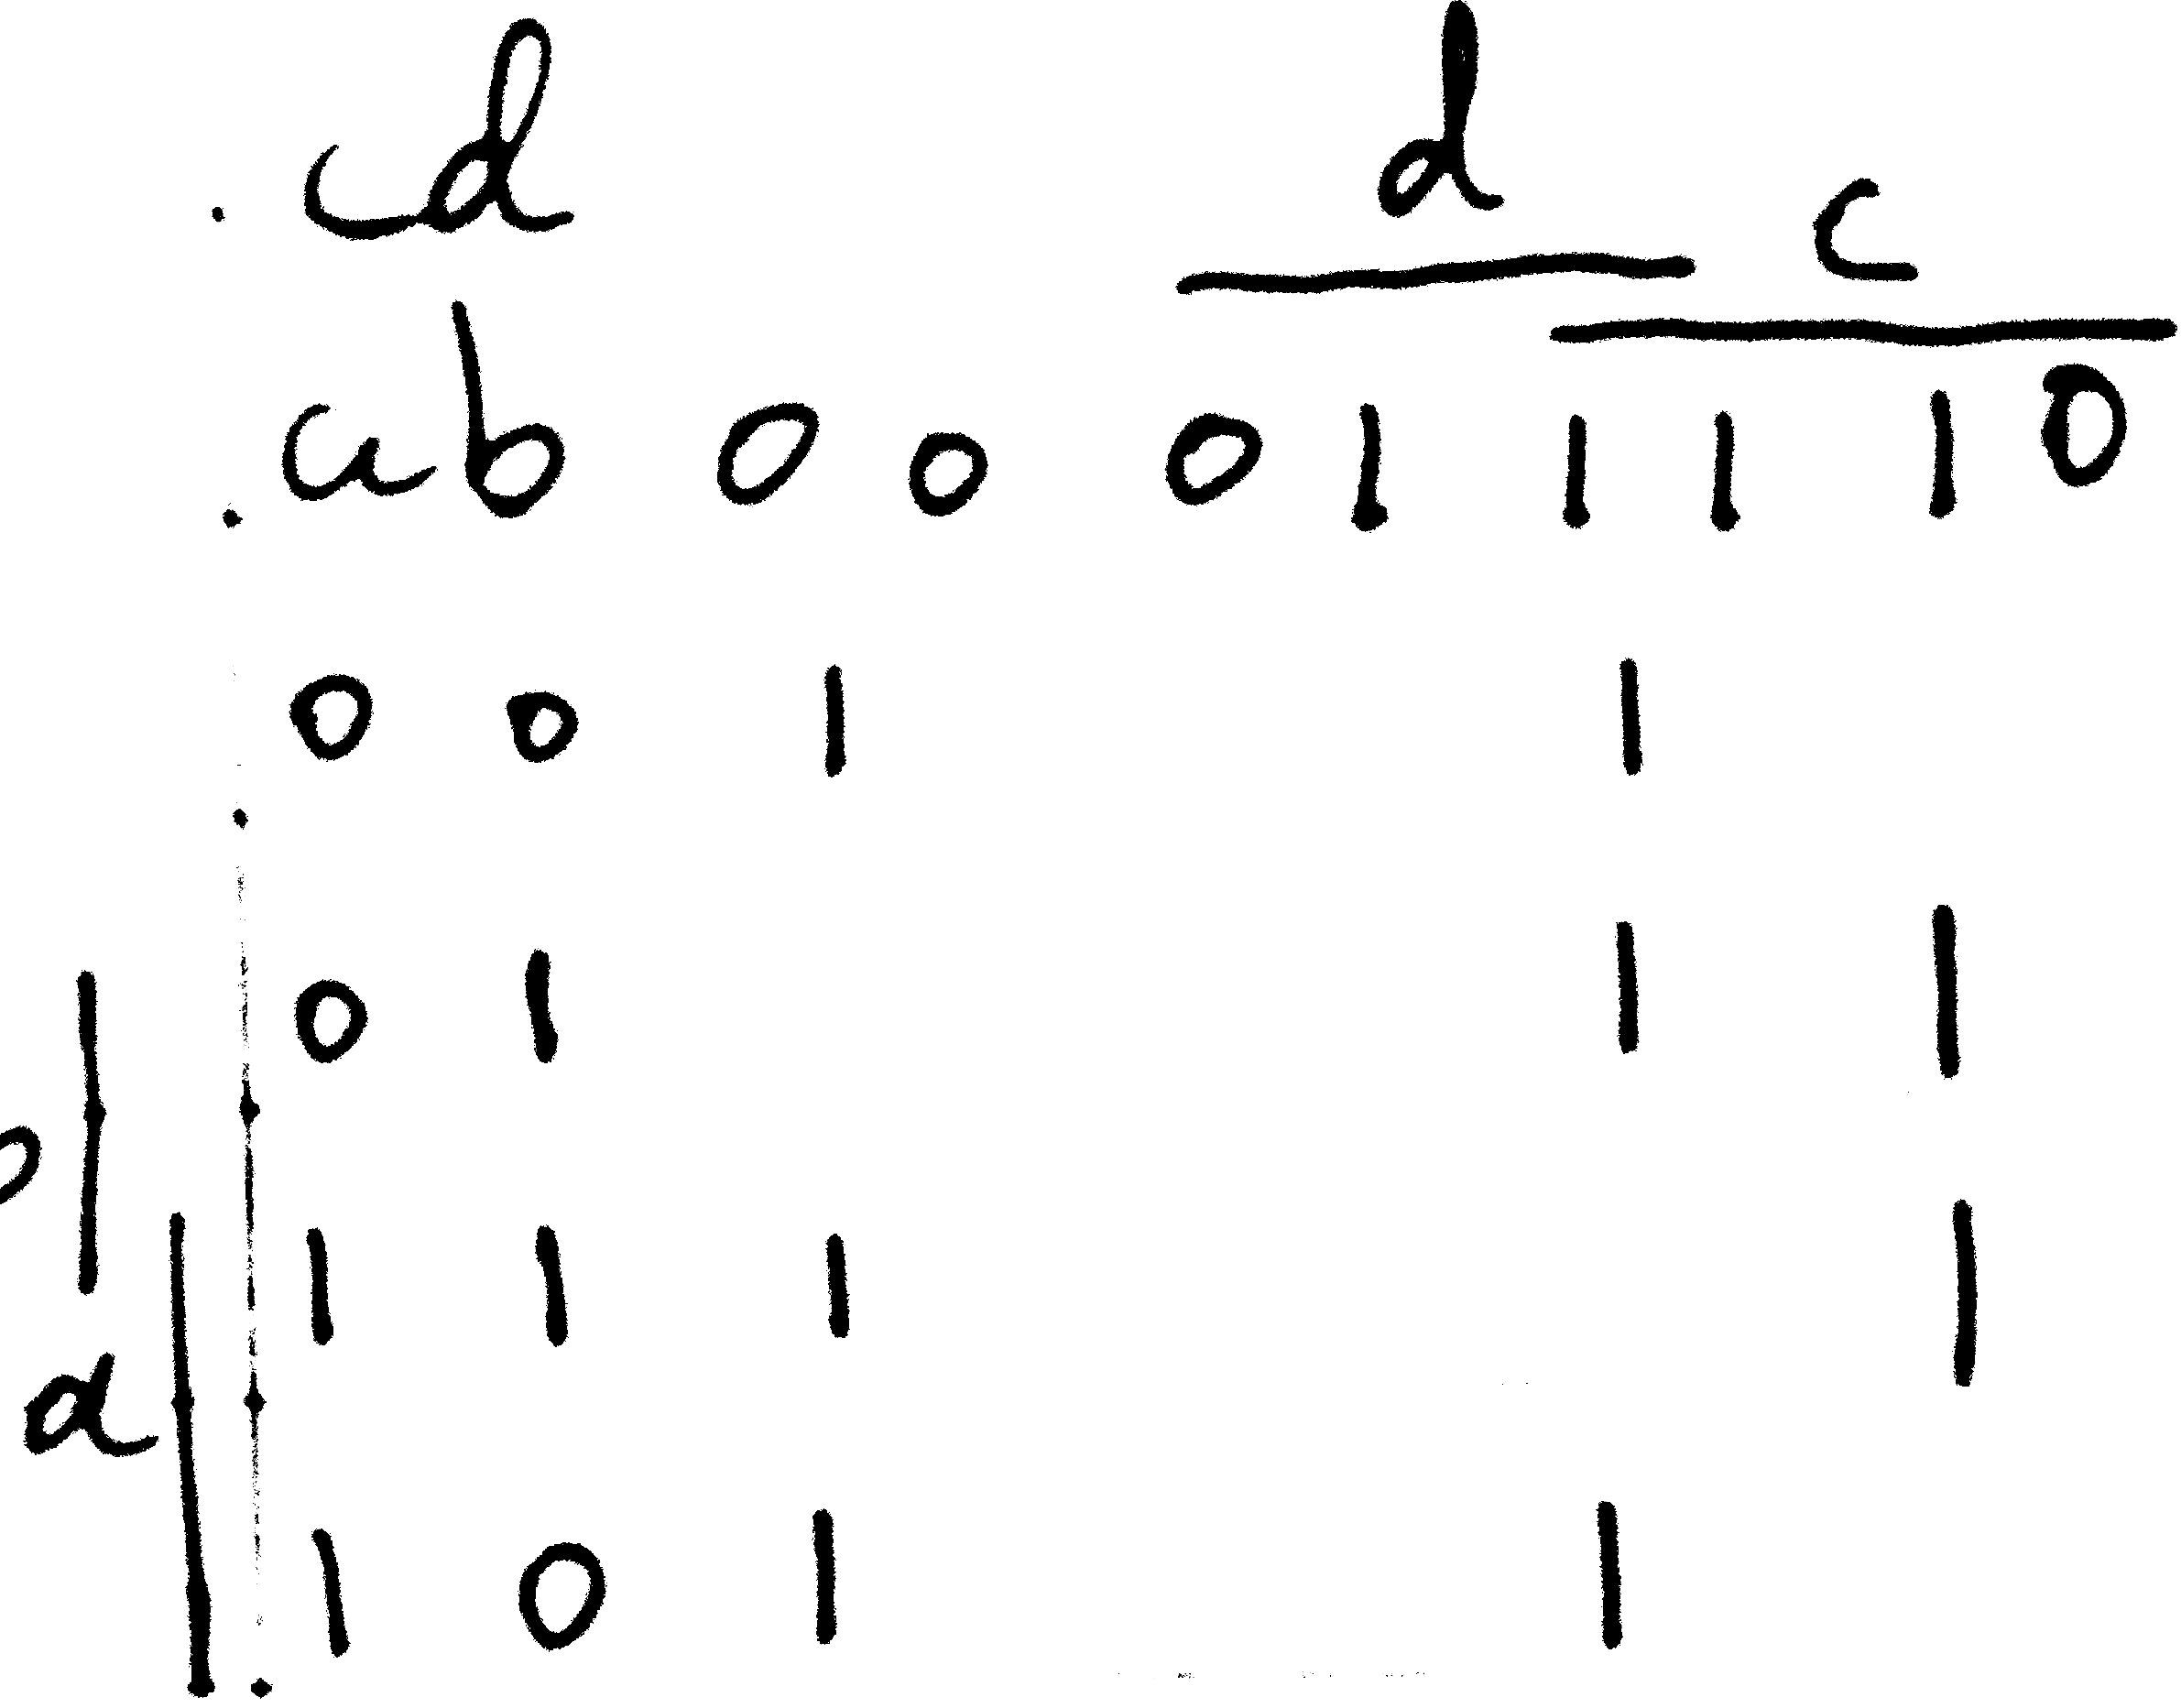
\includegraphics[scale=0.1]{sv2-2-a1.png} 
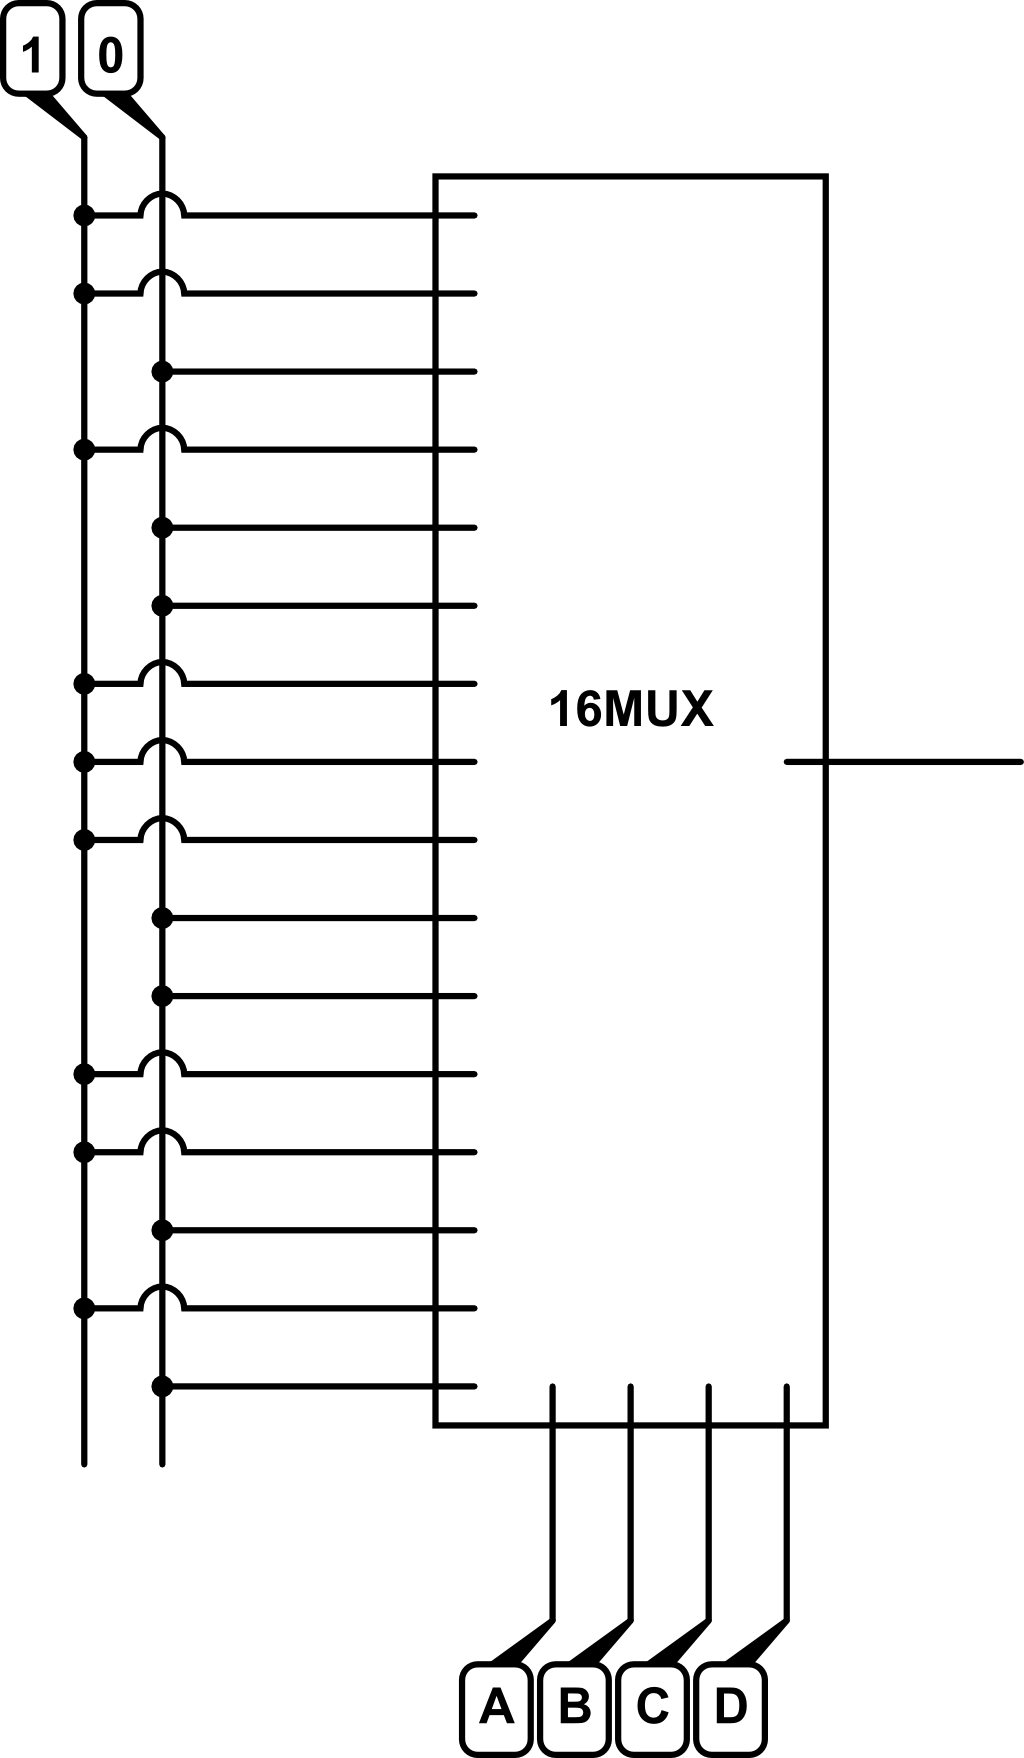
\includegraphics[scale=0.4]{sv2-2-a.png} 

\item[(b)]
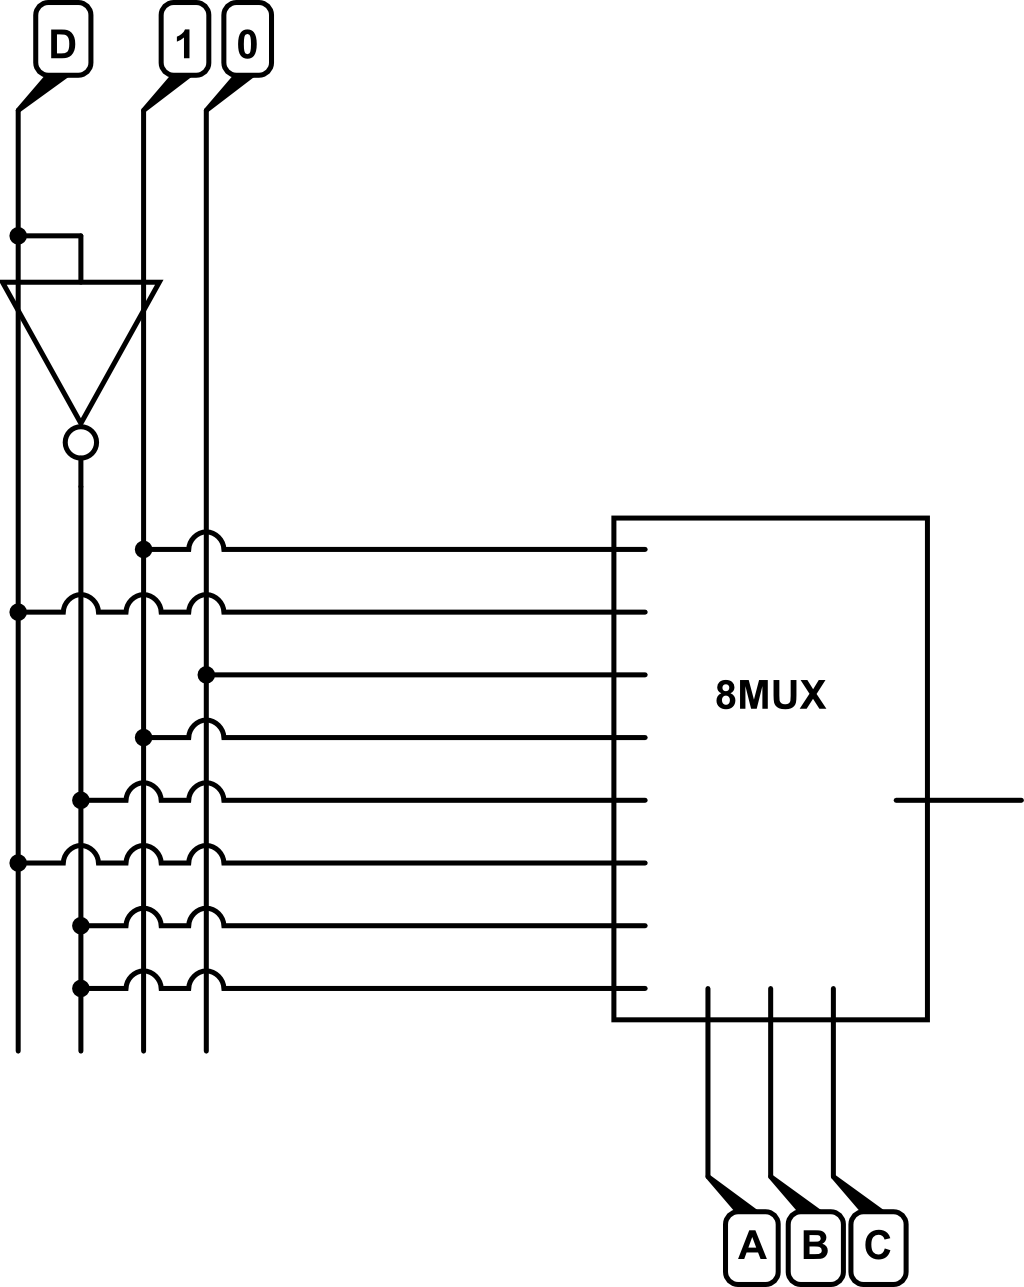
\includegraphics[scale=0.4]{sv2-2-b.png} 
\begin{tabular}{c c c c c c}
A & B & C & D & result & \\
\hline
0&0&0&0&1&1\\
0&0&0&1&1&\\\hhline{----}
0&0&1&0&0&D\\
0&0&1&1&1&\\\hhline{----}
0&1&0&0&0&0\\
0&1&0&1&0&\\\hhline{----}
0&1&1&0&1&1\\
0&1&1&1&1&\\\hhline{----}
1&0&0&0&1&$\bar{D}$\\
1&0&0&1&0&\\\hhline{----}
1&0&1&0&0&D\\
1&0&1&1&1&\\\hhline{----}
1&1&0&0&1&$\bar{D}$\\
1&1&0&1&0&\\\hhline{----}
1&1&1&0&1&$\bar{D}$\\
1&1&1&1&0&\\
\end{tabular}\\
* n means not related with D. \\
Because for specific A,B,C the result is either based on D or $\bar{D}$ or unrelated to D and constrained to 1 or 0. So the D or $\bar{D}$ can be an input instead of control input.

\end{enumerate}

\section*{Exercise 3}



\section*{Exercise 4}
\begin{enumerate}
\item[(a)]
$\bar{B}+C$
\item[(b)]
$ $
\item[(c)]
$\bar{B}+C$
\item[(d)]
$ $
\end{enumerate}
\section*{Exercise 5}
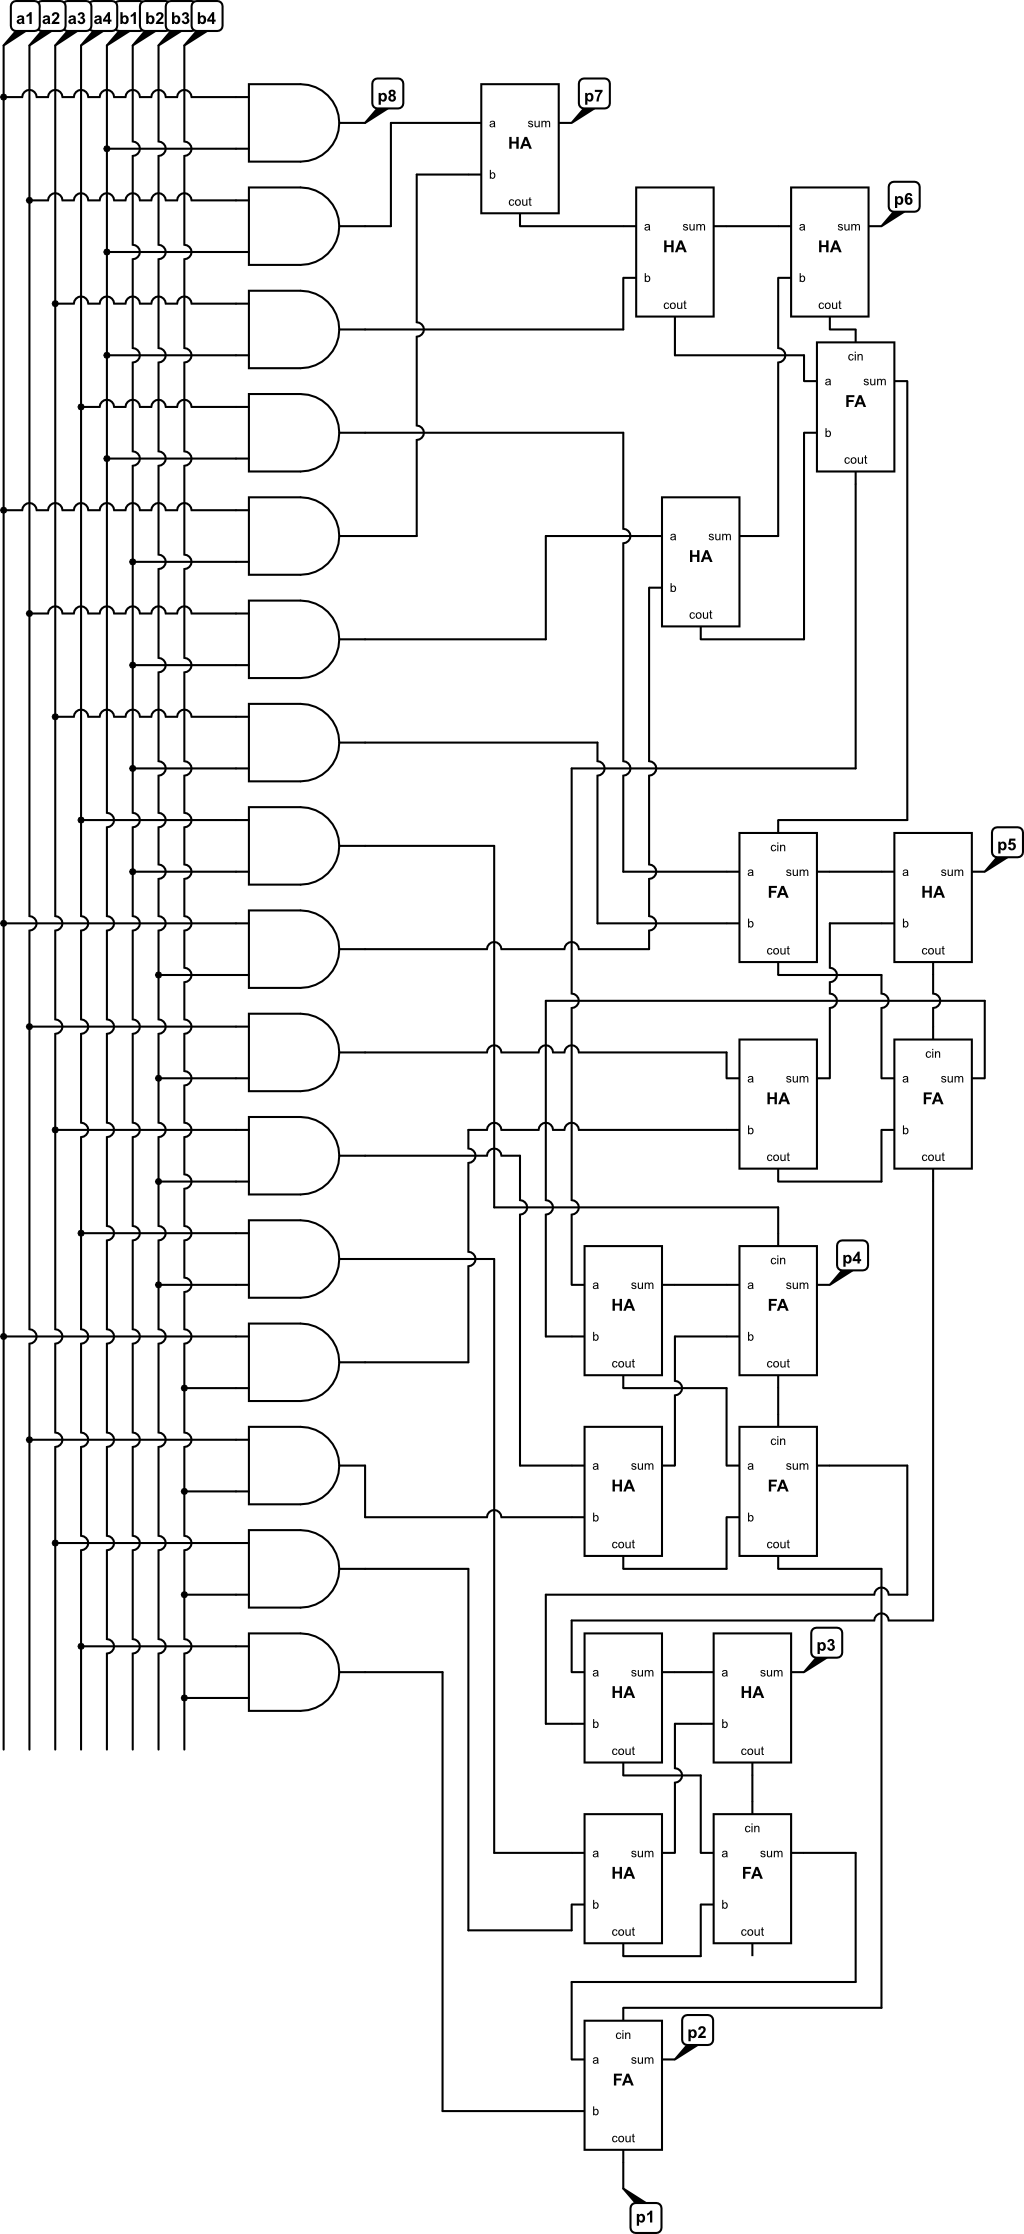
\includegraphics[scale=1]{sv2-5.png}\\
*$x_n$ means the nth number from most significant to least significant of binary number x.\\
This idea comes from the basic product operation by human.
And notice the one of the full adder close to bottom is impossible to have a $c_{out}$ as one.
\section*{Exercise 6}

m means the number of bits in each address.\\
n means the number of input for address looking-up.(So there are $2^n$ different address)\\
Number of bit stored: $m\times 2^n$\\
The ROM is basically a n-input looking-up table for m-bit words. However the implement for PAL is by a SOP formula, the complement or uncomplement of each variable will join in AND gates and then the output of these AND gates will be input to OR gates again to  give an output.

\section*{Exercise 7}

\begin{enumerate}
\item[(i)]
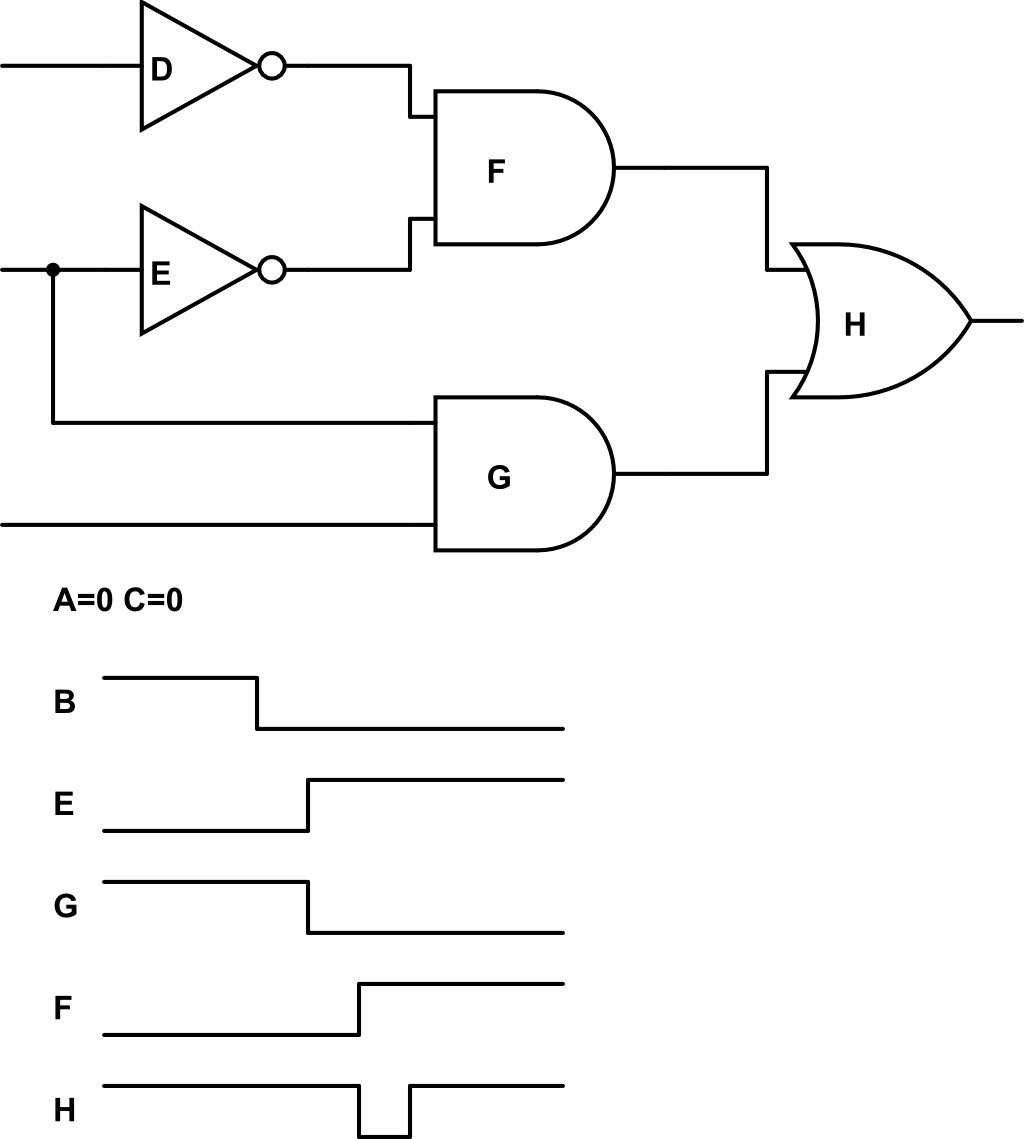
\includegraphics[scale=0.8]{sv2-7-i.png} \\
Propagation delay: $3T$\\
Contamination delay: $2T$

\item[(ii)]
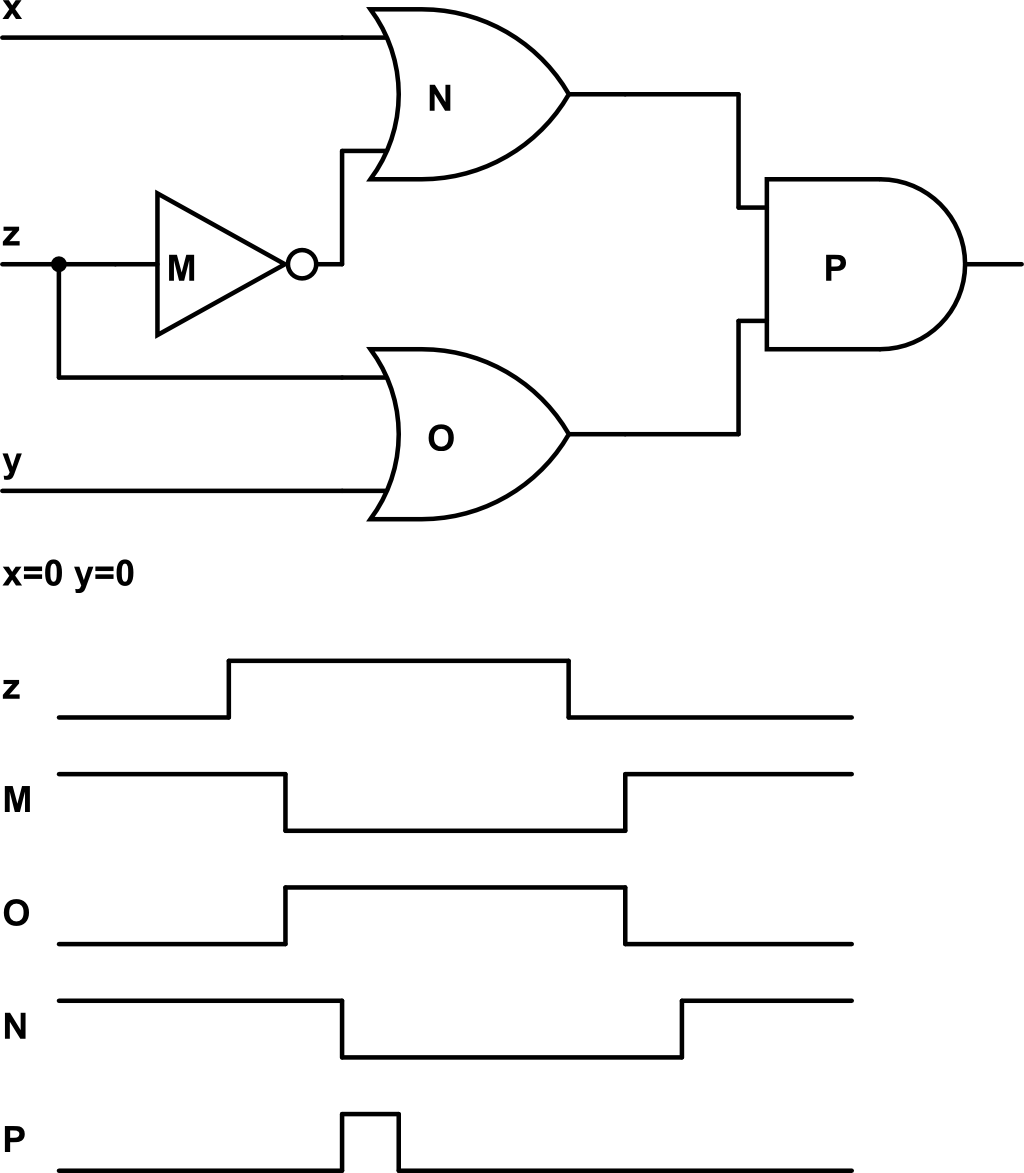
\includegraphics[scale=0.8]{sv2-7-ii.png} \\
Propagation delay: $3T$\\
Contamination delay: $2T$\\
g is a 2-multiplexor
\end{enumerate}

\section*{Exercise 8}
\section*{Exercise 9}
\section*{Exercise 10}
\section*{Exercise 11}
\section*{Exercise 12}
\section*{Exercise 13}
\section*{Exercise 14}
\section*{Exercise 15}
\section*{Exercise 16}
\section*{Exercise 17}
\section*{Exercise 18}

\end{document}

